{ %section3_3
	\subsection{Технология OpenMP}
	\label{OpenMP:section}
	\Large\par\textbf{Краткая характеристика технологии.} Первая версия стандарта OpenMP появилась в 1997 году при поддержке крупнейших IT-компаний мира (Intel, IBM, AMD, HP, Nvidia и др.). Целью нового стандарта было предложить кроссплатформенный инструмент для распараллеливания, который был бы более высокоуровневый, чем API управления потоками, предлагаемые операционной системой. На данный момент OpenMP стандартизована для трёх языков программирования: С, С++ и Фортран.
	\par\textbf{Поддержка компиляторами.} Абсолютное большинство существующих современных компиляторов С/С++ поддерживают OpenMP версии 2.0 (например, как gcc, так и Visual Studio). Однако лишь немногие компиляторы поддерживают более новую версию OpenMP 4.0, поэтому далее при изложении материала будет в качестве "общего знаменателя"\verb+ +использоваться технология OpenMP 2.0.
	\par OpenMP определяет набор директив препроцессору, которые дают указание компилятору заменить следующий за ними исходный код на его параллельную версию с помощью доступных компилятору средств, например с помощью POSIX Threads в Linux или Windows Threads в операционных системах Microsoft. Для корректной трансляции директив необходимо при компиляции указать специальный ключ, значение которого зависит от компилятора (примеры приведены в таблице~\ref{compilerOpenMP:table}).
	\begin{table}[H]
		\Large
		\caption{Ключи компиляторов для запуска OpenMP}
		\label{compilerOpenMP:table}
		\begin{center}
			\begin{tabular}{|c|c|}
				\hline
				\textbf{Название компилятора} & \specialcell{\textbf{Ключ компилятору для включения} \\  \textbf{OpenMP}} \\
				\hline
				Gcc & -fopenmp \\
				\hline
				icc (Intel C/C++ compiler) & -openmp \\
				\hline
				Sun C/C++ compiler & -xopenmp \\
				\hline
				Visual Studio C/C++ compiler & /openmp \\
				\hline
				PGI (Nvidia C/C++ compiler) & -mp \\
				\hline
			\end{tabular}
		\end{center}
	\end{table}
	\parПомимо препроцессорных директив, OpenMP определяет набор библиотечных функций, для вызова которых в исходном коде потребуется подключить заголовочный файл OpenMP:
	\begin{figure}[H]
		
\includegraphics[width=1\linewidth]{includeOpenMP}
	\end{figure}
	\par\textbf{Отличительные особенности.} Среди прочих технологий распараллеливания OpenMP выделяется следующими важными и характеристиками:
	\begin{itemize}
		\itemИнкрементное распараллеливание.
		\itemОбратная совместимость.
		\itemВысокий уровень абстракций.
		\itemНизкий коэффициент трансформации.
		\itemПоддержка крупнейшими  IT-гигантами. 
		\itemАвтоматическое масштабирование.
	\end{itemize}
	\par\textit{Инкрементное распараллеливание.}  OpenMP позволяет распараллеливать существующую последовательную программу в виде  небольших итераций-правок, на каждой из которых будет достигаться всё больший коэффициент распараллеленности программы. Эта особенность является уникальной, т.к. большинство других технологий предполагают существенное изменение структуры распараллеливаемой программы уже на первом этапе процесса распараллеливания, при этом первая работоспособная параллельная версия программы появляется после длительного процесса отладки и программирования новых компонентов, которые неизбежно добавляются при распараллеливании. OpenMP лишён этого недостатка.
	\par\textit{Обратная совместимость.} Большинство программных технологий развиваются с обеспечением обратной совместимости (backward compatibility), когда более новая версия программы поддерживает работоспособность старых файлов. Термин \textit{"прямая совместимость"} (forward compatibility) имеет противоположный смысл: файлы, созданные в программе новой версии, остаются работоспособными при использовании старой версии программы. В случае OpenMP это проявляется в том, что распараллеленная программа будет корректно скомпилирована в однопоточном режиме даже на старом компиляторе, который не поддерживает OpenMP. Важно отметить, что прямая совместимость обеспечивается, если при распараллеливании не используются библиотечные функции OpenMP, а присутствуют только препроцессорные директивы. При наличии библиотечных функций для обеспечения обратной совместимости потребуется написать функции-заглушки в файле "omp.h" (лишь немногие компиляторы умеют генерировать эти заглушки при использовании специального ключа).
	\par\textit{Высокий уровень абстракций.} Одна единственная препроцессораня директива OpenMP после обработки компилятором приводит к существенной трансформации исходной программы с добавлением большого количества новой логики, отвечающей за определение доступного в системе количества процессоров, за запуск и уничтожение потоков, за распределение работы между потоками и т.п. Все эти операции OpenMP берёт на себя,  взамен программист получает набор очень высокоуровневых инструментов распараллеливания. У высокоуровневых языков есть и традиционная тёмная сторона: в OpenMP отсутствует возможность изменить некоторую внутренние детали работы с потоками (например, нельзя установить аффинность  потоков или уменьшить накладные расходы на создание/удаление потоков).
	\par\textit{Низкий коэффициент параллельной трансформации (КПТ).} При распараллеливании существующей последовательной программы приходится вносить в неё достаточно большое количество изменений. Пусть КПТ – это отношение строк нового программного кода, который добавился в результате распараллеливания, к общему количеству строк кода в программе. В OpenMP КПТ обычно существенно ниже, чем у большинства других технологий распараллеливания. Это объясняется высоким уровнем абстракции языка OpenMP (см. предыдущий пункт). 
	\par\textit{Поддержка крупнейшими  IT-гигантами.} Уже при разработке\\ OpenMP о его поддержке заявили крупнейшие игроки IT-мира. Это обеспечило не только высокое качество разработки стандарта, но и наличие готовых реализаций стандарта в популярных компиляторах. Несмотря на прошедшие два десятка лет OpenMP не растерял приверженцев и поддержка новейших версий OpenMP с достаточно малой задержкой появляется в компиляторах. Например, при текущей версии стандарта OpenMP 4.5 наиболее популярные компиляторы уже поддерживают версию OpenMP 4.0. Исключением является только фирма Microsoft. Их компилятор вот уже несколько версий неизменно поддерживает только \\OpenMP 2.0. 
	\par\textit{Автоматическое масштабирование.}  Низкоуровневые технологии распараллеливания (POSIX Threads, OpenCL) предлагают программисту вручную управлять количеством создаваемых потоков при выполнении параллельной работы. Это обеспечивает возможность гибко управлять и настраивать процесс создания потоков в зависимости от количества доступных системе процессоров (ядер), но при этом требует от программиста большой количества неавтоматизируемой работы. В OpenMP управление масштабированием происходит в автоматическом режиме, т.е. OpenMP сам запрашивает у операционной системы количество доступных процессоров и выбирает количество создаваемых потоков. Но при необходимости OpenMP оставляет возможность устанавливать требуемое количество потоков вручную.
	\par\textbf{Примеры OpenMP-программ.} Рассмотрим ниже простейшие примеры работающих параллельных программ, начиная с традиционного для программирования примера "Hello, World":
	\begin{figure}[H]
		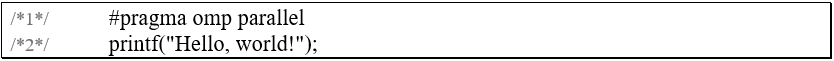
\includegraphics[width=1\linewidth]{OpenMPExample1}
	\end{figure}
	\parРезультатом работы будет выведенное несколько раз в консоль сообщение. Количество сообщений определяется количеством логических процессоров, доступных системе (например, при использовании технологии HyperThreading при двух ядрах количество логических процессоров будет равно четырём). 
	\parДействие директивы pragma распространяется на следующий за ней исполняемый блок. В данном случае это вызов функции printf, но можно было бы заключить произвольное количество операций в фигурные скобки, чтобы расширить исполняемый блок:
	\begin{figure}[H]
		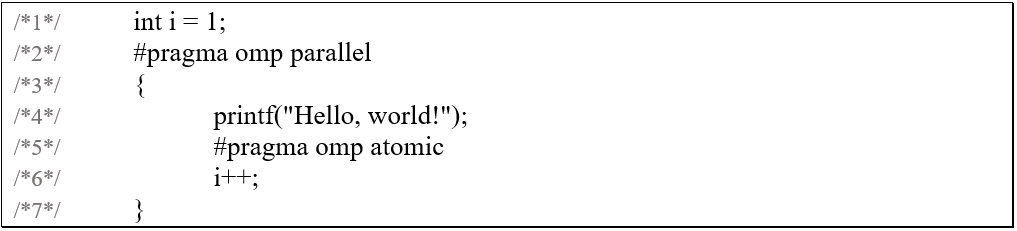
\includegraphics[width=1\linewidth]{OpenMPExample2}
	\end{figure}
	В этой программе заключенный в фигурные скобки блок операций выполняется одновременно на нескольких ядрах. При этом в строке 5 процессору даётся указание выполнить операцию "i++" атомарно, т.е. не параллельно, а последовательно каждым из потоков. 
	\parС одной стороны, это приводит к тому, что операция инкремента перестаёт быть распараллеленной, что снижает скорость многоядерного выполнения. С другой стороны, директива atomic в данном случае необходима, т.к. иначе могла бы возникнуть сложно обнаружимая проблема с гонкой данных, проявляющаяся в конфликте при записи данных в общую область памяти одновременно несколькими потоками в переменную i. Заметим, что директива atomic может применяться только для однострочных простых команд присваивания. 
	\parДля изоляции более сложных составных команд с возможным вызовом пользовательских и системных функций следует использовать директиву critical, которая допускает (в отличие от директивы atomic) возможность расширения своей области действия на блок операций, заключённый в фигурные скобки? при этом каждая critical-секция может иметь имя, позволяющее сгруппировать разные критические секции по этому имени, чтобы предотвратить появление единой распределённой по всей программе критической секции:
	\begin{figure}[H]
		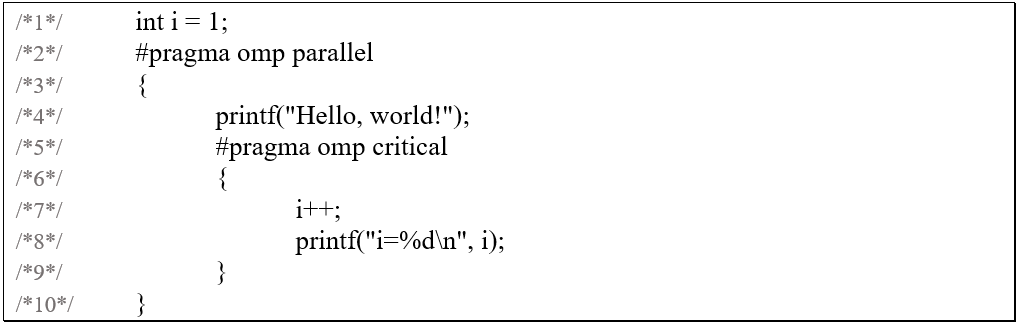
\includegraphics[width=1\linewidth]{OpenMPExample3}
	\end{figure}
	\parВ этом случае функция printf в строке 4 выполняется всеми потоками параллельно, что может привести к перемешиванию выводимых символов. Напротив, функция printf в строке 8 выполняется потоками строго по очереди, что предотвращает возможные конфликты между ними, однако замедляет выполнение программы из-за искусственного ограничения коэффициента распараллеленности.
	\parПриведём пример распараллеливания программы, содержащей последовательный вызов функций run\textunderscore function1 и run\textunderscore function2, которые не зависят друг от друга (т.е. не используют общих данных и результаты работы одной не влияют на результаты работы другой) и поэтому допускающих удобное \textit{распараллеливание по инструкциям} в чистом виде:
	\begin{figure}[H]
		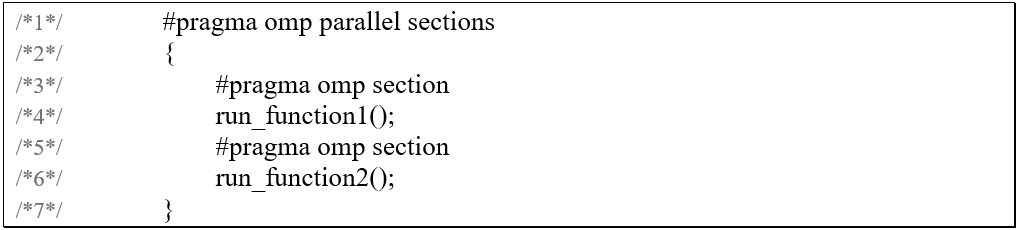
\includegraphics[width=1\linewidth]{OpenMPExample4}
	\end{figure}
	\parРассмотрим пример распараллеливания цикла с использованием OpenMP. Пусть в каждую ячейку одномерного массива нужно записать индекс этой ячейки, возведённый в шестую степень:
	\begin{figure}[H]
		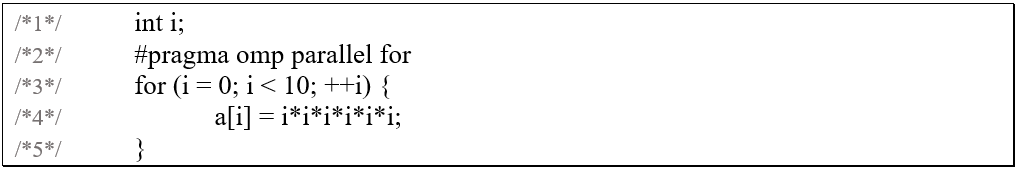
\includegraphics[width=1\linewidth]{OpenMPExample5}
	\end{figure}
	\parПусть указанная программа выполняется на двухъядерном процессоре. Тогда первый процессор рассчитает значения с a[0] по a[4], второй процессор – значения с a[5] по a[9]. Видимо, что при записи в массив процессору не мешают друг другу, т.к. работают с разными частями массива. Попробуем оптимизировать предыдущий вариант, сократив количество операций умножения для возведения в шестую степень:
	\begin{figure}[H]
		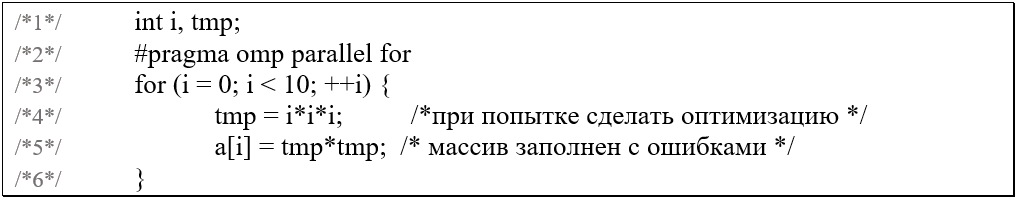
\includegraphics[width=1\linewidth]{OpenMPExample6}
	\end{figure}
	\parВ указанном случае программа будет корректно работать только при наличии одного процессора (ядра). При наличии нескольких ядер будет наблюдаться состояние гонки данных при одновременной записи нового значения в переменную tmp (строка 4) несколькими потоками, в результате массив будет заполнен некорректно. Например, пусть первый поток, выполняющий итерацию i=2 записал в tmp число 8. Теперь при вычислении a[2] поток попытается записать число 8*8, однако если до начала строки 5 успеет вклиниться второй поток, работающей с итерацией i=7, то значение tmp превратиться в 7*7*7, а значение a[2], рассчитываемое первым потоком, превратиться в $7^6$, вместо положенных 64. Исправим допущенную ошибку следующим образом:
	\begin{figure}[H]
		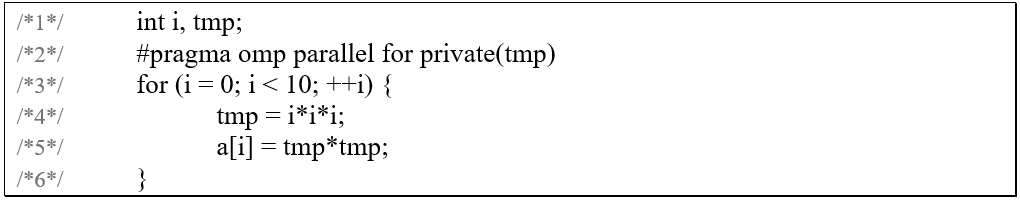
\includegraphics[width=1\linewidth]{OpenMPExample7}
	\end{figure}
	\parВ директиве препроцессору появился новый элемент: private. Этот элемент задаёт через запятую перечень локальных (приватных) для каждого потока переменных. В данном случае такая переменная одна: tmp. Другой равноценный способ исправить ошибку – это перенести объявление переменной "int tmp" внутрь параллельной области, что заставить OpenMP считать эту переменную локальной для каждого потока. Может возникнуть вопрос, почему в перечень локальных переменных не добавлена i. Ответ не очевиден: OpenMP по умолчанию считает переменную распараллеливаемого цикла локальной.
	\parЛюбая переменная, объявленная внутри параллельной области, считается в OpenMP локальной, поэтому такие переменные не нужно указывать в списке. Любая переменная, объявленная вне этой области является глобальной (в нашем случае глобальной переменной является указатель на массив а. Но если хочется явным образом указать на глобальность переменной, следует рядом с командой private использовать команду shared(x,\ldots), где x задаёт список глобальных переменных.
	\parРассмотрим пример, в котором нужно рассчитать сумму и произведение элементов следующего ряда: $\{\;1^i,\;2^i,\;3^i,\;4^i,\;5^i\;\}$ для различных значений $i$, например: $i\;=\;1,\;2,\;3$. Приведём ниже решение поставленной задачи, но умышленно допустим в ней ошибку:
	\begin{figure}[H]
		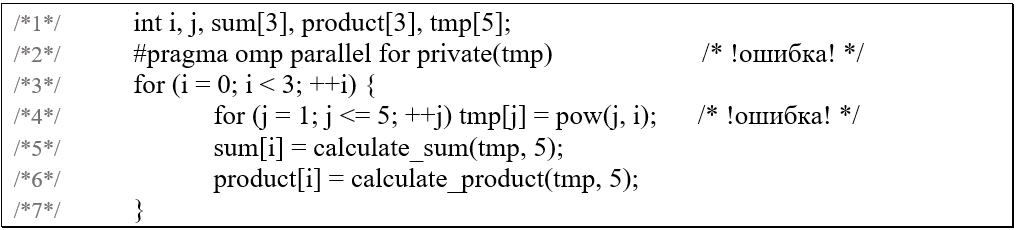
\includegraphics[width=1\linewidth]{OpenMPExample8}
	\end{figure}
	\parВ строке 2 происходит запуск параллельной области, но программист забывает указать, что переменные j и массив tmp должны быть локальными для каждого треда. Действительно, в строке 10 происходит инкремент общей для потоков переменной j, который выполняется всеми потоками одновременно. В этой ситуации потоки могут помешать друг другу, переписав чужое значение j. Исправим обе ошибки следующим образом:
	\begin{figure}[H]
		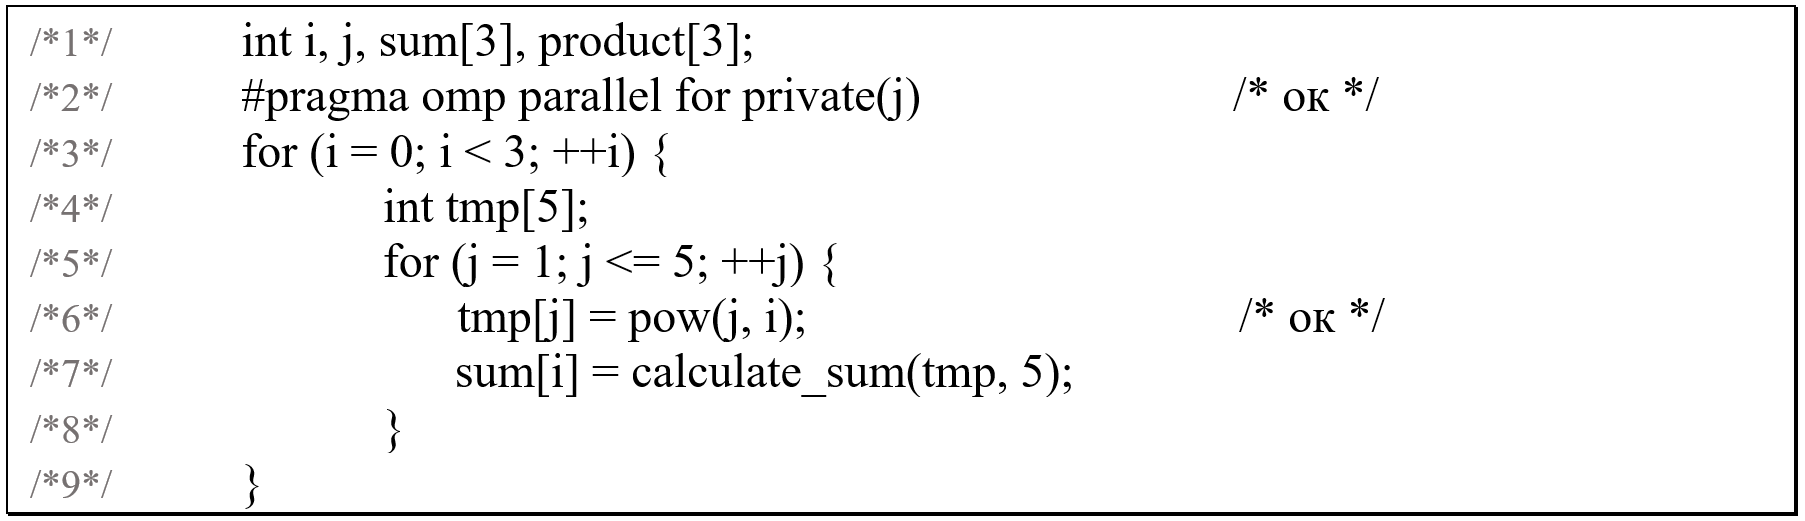
\includegraphics[width=1\linewidth]{OpenMPExample9}
	\end{figure}
	\parВидим, что теперь переменная j явным образом обозначена локальной (private). С массивом tmp решение другое – он весь помещается внутрь параллельной области (т.е. у каждого потока будет свой собственный не зависимый от других экземпляр массива tmp). Почему же нельзя было просто указать переменную tmp в перечне команды private, как это было сделано для j? Ответ связан со спецификой языка С: переменная tmp является указателем, который при работе цикла не меняется, но меняется содержимое памяти, на которое указывает tmp. Это значит, что указыание tmp в качестве private-переменной не решило бы проблему с гонками данных, т.к. все потоки получили бы один и тот же адрес tmp и мешали бы друг другу, записывая новые значения по этому адресу.
	\parРассмотрим ещё одну типичную для параллельного программирования ошибку. Следующая программа считает сумму чисел от 1 до 100:
	\begin{figure}[H]
		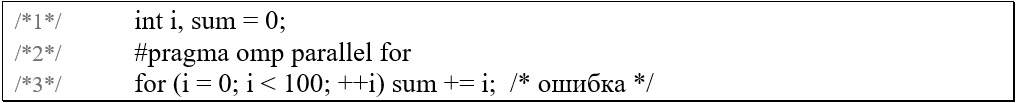
\includegraphics[width=1\linewidth]{OpenMPExample10}
	\end{figure}
	\parПеременная sum является глобальной, поэтому при попытке записать в неё новое значение потоки будут мешать друг другу. Чтобы исправить ошибку, нам придётся использовать локальную для каждого потока сумму, а затем потребуется сложить все эти локальные суммы:
	\begin{figure}[H]
		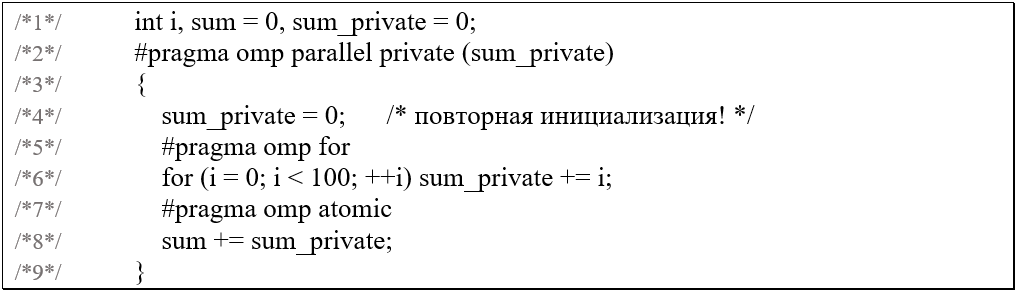
\includegraphics[width=1\linewidth]{OpenMPExample11}
	\end{figure}
	Видим начало параллельной области в строке 2 – именно в этом месте OpenMP создаёт несколько потоков. В строке 6 новые потоки не создаются (т.к. отсутствует ключевое слово parallel), но входящие в цикл потоке делят итерации между собой, а не выполняют каждый все итерации целиком. В строке 8 рассчитавший свою частичную сумму поток пытается прибавить эту сумму к общей сумме. Это приходится делать с помощью директивы atomic, которая гарантирует, что потоки не будут мешать друг другу при перезаписи sum. 
	\parЕщё один сложный момент – это повторная инициализация переменной sum\textunderscore private в строке 4: необходимость в этом возникает, т.к. OpenMP не инициализирует локальные переменные, даже если есть глобальные переменные с идентичными именами. Подобное решение призвано уменьшить накладные расходы на копирование переменных.
	\parОписанный подход является работоспособным, однако он почти не используется на практике, т.к. стандарт OpenMP для целого класса подобных задач предлагает более высокоуровневое и простое решение. Оно состоит в использовании команды reduction:
	\begin{figure}[H]
		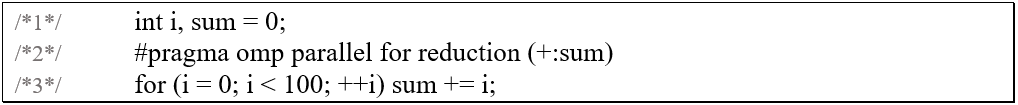
\includegraphics[width=1\linewidth]{OpenMPExample12}
	\end{figure}
	\parКоманда reduction помечает перечисленный переменные как локальные, а в конце параллельной области все локальные переменные объединяет (агрегирует) в одну глобальную переменную с тем же именем, используя указанную операцию. В нашем случае операцией является суммирование. Но OpenMP допускает вместо знака "\verb+++"\verb+ + использовать \verb+"*"+, \verb+"-"+, \verb+"/"+. Важно, что reduction кроме прочего выполняет инициализацию переменных не значениями исходных глобальных переменных, а наиболее соответствующими логики агрегации значениями: например, при суммировании переменная инициализируется нулём, а при умножение – единицей.
	\parПри распараллеливании цикла может оказаться, что итерации неравноценные по количеству выполняемой работы между собой. Это может привести к тому, что один поток справится с выделенной половиной итераций намного быстрее второго потока и будет простаивать. Для решения этой проблемы OpenMP предлагает четыре разных способа распределения итераций по потокам. 
	\begin{itemize}
		\item\textit{Способ по умолчанию:} при этом итерации делятся на количество частей, равное количеству потоков; каждый поток выполняет после этого свою часть и не может взять чужую работу.
		\item\textit{Статическое распределение (static):} итерации разбиваются на части указанного пользователям размера; затем ещё до начала работы каждый поток получает фиксированное количество частей и выполняет только их без возможности переключиться на другие.
		\item\textit{Динамическое распределение (dynamic):} итерации разбиваются на части указанного пользователям размера; затем сразу начинается работа цикла и каждый поток получает новую часть итераций по мере завершения работы над предыдущей.
		\item\textit{Управляемое распределение (guided):} компилятор разбивает итерации на количество частей, равное удвоенному количеству потоков; затем сразу начинается работа цикла и каждый поток получает новую часть итераций по мере завершения работы над предыдущей, при этом размер нововыданной части уменьшается по сравнению с предыдущим разом, но не может стать меньше указанного пользователем константного значения.
	\end{itemize}
	\parУпомянутый в каждом из методов пользовательский параметр называется chunk\textunderscore size. Каждый из указанных методов имеет свою область применения, в которой он может обеспечить максимальное параллельное ускорение. Отметим, что режимы dynamic и guided несмотря на свою логичность имеют и свои недостатки: они требуют существенных накладных расходов во время работы цикла по сравнению со static. Также важно понимать, что при выборе числа
	\parРассмотрим пример статического распределения итераций:
	\begin{figure}[H]
		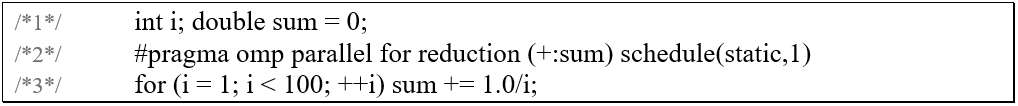
\includegraphics[width=1\linewidth]{OpenMPExample13}
	\end{figure}
	\parПри наличии трёх ядер OpenMP создаст три потока. Первому потоку достанутся итерации $i=1,\;4,\;7,\;…,\;97$ второму – итерации $i=2,\;5,\;8,\;…,\;98$, третьему – итерации $i=3,\;6,\;9,\;…,\;99$. Обратим внимание, что выбор малого значения параметра chunk\textunderscore size = 1 в данном случае не имеет каких-либо негативных эффектов. Однако если бы i использовалась в качестве индекса при обращении к массиву, то предложенный вариант разбиения привёл бы к обращению в память не подряд по последовательным адресам, а разреженно с шагом 3, что ухудшило бы показатели cache hit при использовании кэширования.
	\parРассмотрим ещё один пример: 
	\begin{figure}[H]
		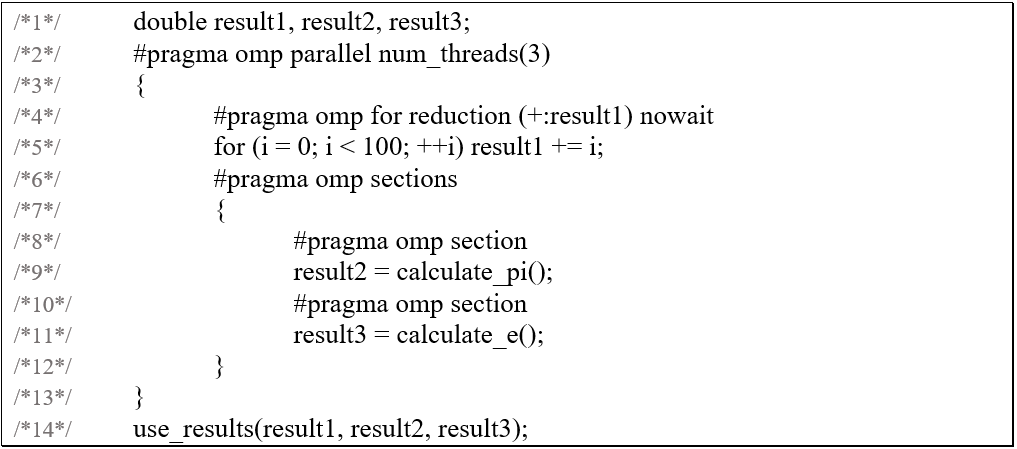
\includegraphics[width=1\linewidth]{OpenMPExample14}
	\end{figure}
	\parЗдесь приводится пример, как можно указать OpenMP количество создаваемых потоков с помощью опции num\textunderscore threads (строка 2), не ориентируясь на реально доступное количество ядер (процессоров) на компьютере. Далее три созданных потока делят между собой 100 итераций уже знакомым нам способом. Однако опция nowait позволяет первому справившемуся с работой потоку не дожидаться остальных, а перейти к следующей за циклом работе. За циклом в параллельном режиме выполняются две функции (строки 9 и 11). Каждая из функций заключена в секцию (section), которые должны иметь родительский элемент sections. В итоге первый освободившийся после цикла поток займётся вычислением функции в строке 9. Второй освободившийся поток вычислит функцию в строке 11. Третьему потоку не достанется работы помимо своей доли итераций в первом цикле.
Общим требованием OpenMP к распараллеливаемым циклам является их \textit{каноничность}. Цикл for называется \textit{каноническим}, если можно при его начале заранее рассчитать количество предстоящих итераций. Это возможно, если одновременно выполняются следующие условия:
	\begin{itemize}
		\itemвнутри цикла нет операций break и return;
		\itemвнутри цикла нет операции goto, ведущей вовне цикла;
		\itemпеременная цикла (итератор) не изменяется внутри цикла;
	\end{itemize}
	При этом запись цикла должна иметь вид "for (i = A; i < B; i+=C)\verb+"+, где числа A, B, C не должны меняться во время работы цикла. При этом второй параметр цикла может использовать не только знак "меньше", но и  \verb+">"+,  \verb+">="+,  \verb+"<="+. Третий параметр цикла может не только инкрементировать, но декрементировать переменную цикла (допускается краткая форма записи   \verb|"i++"|).
	\parЕсли итерация k влияет на результаты итерации m, то цикл нельзя распараллеливать, т.к. нельзя заранее предсказать порядок завершения итераций несколькими потоками.  Ответственность за обнаружение таких конфликтов лежит на программисте. Например, OpenMP не обнаружит взаимозависимость итераций и скомпилирует следующую программу:
	\begin{figure}[H]
		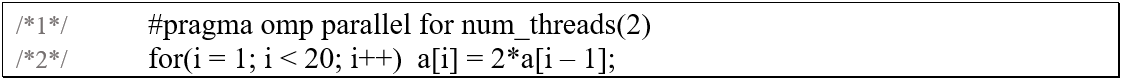
\includegraphics[width=1\linewidth]{OpenMPExample15}
	\end{figure}
	\parВ этой программе поток 0 скорее всего не успеет заполнить элемент a[9] к тому моменту, когда поток 1 будет вычислять значение a[10] = 2*a[9].
	\par
}